\chapter{Computations and Readout}\label{chap:computations_and_readout}
To control and do read out of a superconducting qubit, it is coupled to both several feed lines and a resonator. In this section, we will cover the theory of how a qubit is controlled and how the coupling allows us to do dispersive readout of the qubit.

\section{Qubit Control}\label{sec:qubit_control}
The state of the qubit is modelled as a two level system and can be visualized as a vector on the Bloch sphere. In this view, any qubit operation can be thought of a rotation around the sphere. While we need two angles to represent a state, we need three to describe an arbitary rotation.\footnote{Since a rotation consist of an axis (a vector represented by two angles $\theta, \phi$) and an angle, $\psi$, determining how much we rotate around that axis, we need in total the three values $\theta, \phi$ and $\psi$ to describe the arbitary rotation.}

To describe all the rotation, we thus need the identity and three generators of rotations. This is called a \textit{Universal Gate Set} for one qubit, from which every other rotation/unitary transformation can be build. A common representation is to choose the Pauli gate set consisting of $\{\identity, \sigma_x, \sigma_y, \sigma_z\}$:
\begin{fullwidth}
\begin{equation}
    \identity = \begin{pmatrix}
        1 & 0 \\ 
        0 & 1
    \end{pmatrix}, \quad
    \sigma_x = \begin{pmatrix}
        0 & 1 \\ 
        1 & 0
    \end{pmatrix}, \quad
    \sigma_y = i\begin{pmatrix}
        0 & -1 \\ 
        1 & 0
    \end{pmatrix}, \quad
    \sigma_z = \begin{pmatrix}
        1 & 0 \\ 
        0 & -1
    \end{pmatrix}, \quad
\end{equation}
\end{fullwidth}
these gates are also considered the generators of the gates, since the rotations are made by taking the exponential of the gates. An example is a $\pi/2$ rotation around the $x$-axis is made by:
\begin{equation}
    R_X^{\pi/2} = e^{i \frac{\pi}{2} \hat{X}} = \frac{1}{\sqrt{2}}\begin{pmatrix}
        1  & -i \\
        -i & 1
    \end{pmatrix} 
\end{equation}
which sends the $\ket{0}$ to $\frac{1}{\sqrt{2}}(\ket{0} - i\ket{1})$, a state along the y-axis. 
When comparing this to the time evolution described in section \ref{sec: Time Evolution}, the gates correspond to the Hamiltonian and by applying the gate a certain amount of time, we can adjust the angle of the rotation. To completely control a qubit, the goal is now clearer: we need the ability to apply a full gate set to a qubit, which can be done by adding terms to the Hamiltonian. 

If we were to further extend the scope to multi qubit gates, we would also need one fully-entangling two qubit gate to have complete the Universal Gate Set. Most commonly, this would be the Control-Not or a Control-phase gate, but we will only consider one qubit in this thesis \cite{krantz_quantum_2019}.


\subsection{Capacitative Coupling}
By running a voltage line to the qubit and coupling it capacitatively, we couple to the charge in the qubit. This adds a term proportional $\hat{n}V(t)$ to the Hamiltonian, where the factors are given by the capacitance of the device and the capacitor coupling them. If we were to consider the charge matrix in the energy basis of the LC-basis (harmonic oscillator), it can be decomposed into $n \propto -i(a - a^\dagger)$ coupling the different energy levels. While the transmon Hamiltonian differs a bit from the LC-circuit its diagonal terms of $\mel{k}{n}{k} = 0$ and only the off diagonal elements remain. Applying the same logic\footnote{Which is a bit of stretch because of the anharmonicity, but it works out when we truncate to only two energy levels. For higher level terms, we calculate the $n$ operator in the energy basis and use that operator instead of this approximation.}, we can get $n \propto i(\sigma_+ - \sigma_-)$ for the qubit as well. Here $\sigma_+ = \ket{1}\bra{0}$ and $\sigma_- = \ket{0}\bra{1}$ \cite{krantz_quantum_2019}. The applied voltage gives a contributions to the Hamiltonian of the form:
\begin{equation}
    H_{QD} = - \Omega(t) i \left(\sigma_+ - \sigma_- \right) = \Omega(t) \sigma_y
\end{equation}
Where $\Omega(t)$ consist of our controlled voltage along with a scaling dependent on the coupling to qubit.  

\subsection{The Qubit in the Interaction Picture}
A truncated qubit in its eigenbasis has the Hamiltonian:
\begin{equation}
    H = \frac{1}{2} \omega_{q} \sigma_z
\end{equation}
where the $\omega_q = \omega_{01} = E_1 - E_0$ (where we still omit the factor of $\hbar$). After adding the contribution from the control line, we have:
\begin{equation}
    H = \frac{1}{2} \hbar \omega_{q} \sigma_z + \Omega V(t) \sigma_y
\end{equation}
To go into the interaction picture, we consider $H_0 = \frac{1}{2} \omega_{q} \sigma_z$ and $H_d = \Omega V(t) \sigma_y$, such that the full Hamiltonian is $H = H_0 + H_d$. The transformation to the rotating is:
\begin{equation}
    \ket{\psi} \to \ket{\tilde{\psi}} = \mathcal{U}(t)\ket{\psi}, \quad \text{with}\quad \unitary(t) = e^{iH_0 t}
\end{equation}
In this basis, the Schrödinger equation becomes:
\begin{align*}
    i\partial_t \ket{\tilde{\psi}(t)} &= i \partial_t (\mathcal{U}(t) \ket{{\psi}(t)}) \\
    &= i \dot{\mathcal{U}}(t)\ket{\psi(t)} + i \mathcal{U}(t) {\ket{\Dot{{\psi}}(t)}}
\end{align*}
And using the original Schrödinger equation:$\partial_t\ket{\psi(t)} = i H \ket{\psi}$ and the transformed state $\ket{\psi(t)} = \mathcal{U}^\dagger(t) \ket{\tilde{\psi}(t)}$, we get:
\begin{equation}
    i \partial_t \ket{\Tilde{\psi}(t)}= \left[(\dot{i \mathcal{U}}{(t)}\unitary^\dagger(t) + \unitary(t) H \unitary^\dagger(t)\right]\ket{\tilde{\psi}(t)}
\end{equation}
Such that the effective Hamiltonian in the rotating frame is given as:
\begin{equation}
    H_{eff} = \dot{i \mathcal{U}}{(t)}\unitary^\dagger(t)) + \unitary(t) H \unitary^\dagger(t)
\end{equation}
or in the case of the rotating frame of the qubit:
\begin{equation}
    H_{eff} = - H_0 + H_0 + \unitary(t) H_d \unitary^\dagger(t)
\end{equation}
where we have used that the transformation is unitary $\unitary^\dagger \unitary = \identity$ and that it commutes with $H_0$ $\comm{\unitary}{H_0} = 0$. Substituting $H_D$ and $\unitary(t)$ we get\footnote{Writing $\sigma_y = i (\ket{1}\bra{0} - \ket{0}\bra{1})$ makes this calculation much easier.}\cite{krantz_quantum_2019}:

\begin{fullwidth}
\begin{align}
    H_{eff} &= \Omega V(t) i \exp\left(it\frac{\omega_q \sigma_z}{2}\right)  (\ket{1}\bra{0} - \ket{0}\bra{1} )\exp\left(-it\frac{\omega_q \sigma_z}{2}\right) \\
            &= \Omega V(t) i \left(e^{-it\omega_q}\ket{0}\bra{1} -  e^{+it\omega_q}\ket{1}\bra{0} \right) \\
            &= \Omega V(t) i \left(\left(\cos(\omega_q t) - i\sin(\omega_q t)\right)\ket{0}\bra{1} -  \left(\cos(\omega_q t) + i\sin(\omega_q t)\right)\ket{1}\bra{0} \right) \\
            &= \Omega V(t) \left(\cos(\omega_q t)\sigma_y - \sin(\omega_q t) \sigma_x \right)
\end{align}
\end{fullwidth}
Here we see that in the rotating frame, we get both a contribution of $\sigma_x$ and $\sigma_y$ \cite{krantz_quantum_2019}. 

\subsection{X, Y and virtual Z}\label{sec:how_to_make_gates}
To arrive at the gates, we consider the qubit in its rotating frame. Now we apply a pulse through the control line. Normmally this will have an oscillating term and an envelope:
\begin{equation}
    V(t) = s(t) (\sin(\omega_d t + \phi))
\end{equation}
where $s(t)$ is the envelope of our pulse with driving frequency $\omega_d$ and phase shift $\phi$. By defining $I = \cos(\phi), Q = \sin(\phi)$, the pulse can be written as:
\begin{equation}
    V(t) = s(t) \left(I \cos(\omega_d t) + Q \sin(\omega_d t)\right) 
\end{equation}
Such that the effective driving Hamiltonian becomes:
\begin{fullwidth}
\begin{equation}
    H_{eff} = \Omega s(t) \left(I \cos(\omega_d t) + Q \sin(\omega_d t)\right)   \left(\cos(\omega_q t)\sigma_y - \sin(\omega_q t) \sigma_x \right)
\end{equation}
\end{fullwidth}
It is now time to perform the infamous rotating wave approximation (RWA). The basic idea is to decompose our Hamiltonian into fast and slow oscillating term $H = H_{slow}(t) + H_{fast}(t)$. The time evolution operator becomes\footnote{Here we assume that the Hamiltonian commutes with itself at different times, which is the case for the one we are dealing with} $\unitary(t) = \exp(i\int_0^tdt'H_{slow}(t') + i\int_0^tdt'H_{fast}(t'))$, but at any oscillation rate were the slow oscillating term gives a non-vanishing value, the fast oscillating term will cancel in the integral. We thus get $\unitary(t) \approx \exp(i\int_0^tdt'H_{slow}(t'))$ and for relevant dynamics, we can just consider $H\approx H_{slow}(t)$. 
% \todo{Tighten this section, it is because it averages, maybe also check the footnote with Sakurai}
\sidenote[][-0.5 cm]{This works as the time-evolution operator is given by $U = \exp(i\int dt H)$ so fast oscillating term will cancel if the time interval is sufficiently large.}
Rewriting the Hamiltonian with the product to sum trigonometric identities\sidenote[][-0.0 cm]{An example is the $\cos(\alpha)\cos(\beta)=\frac{1}{2}(\cos(\alpha-\beta) + \cos(\alpha + \beta))$}, one would get: 

\begin{fullwidth}
    
\begin{align}
H_{eff} &= \Omega s(t) \left((I \cos(\omega_d t) + Q \sin(\omega_d t)) \cdot \cos(\omega_q t)\sigma_y - \left(I \cos(\omega_d t) + Q \sin(\omega_d t)\right) \cdot \sin(\omega_q t) \sigma_x \right) \\
H_{eff} &\approx \Omega s(t) \left((-I \cos(\delta t) + Q \sin(\delta t))\sigma_y + \left(I \cos(\delta t) - Q \sin(\delta t)\right) \sigma_x \right)
\end{align}
\end{fullwidth}
where $\delta = \omega_q - \omega_d$ and the RWA was applied in the the second line to eliminate fast oscillating terms of frequency $\omega_q + \omega_d \gg \omega_q - \omega_d$. In our driving hardware, we can control the driving frequency, the phase $\phi$ and by extension $I$ and $Q$. If we want to perform an x-gate, we can set$I = 1, Q = 0$ and drive the qubit at the qubit frequency $\delta = 0$. The $y$-gate is done exactly the same, but at a $\pi/2$ rotation, such that $I = 0, Q = 1$. 
To complete our 1-qubit universal gate set, we now just need the $\sigma_z$ gate. Since $\sigma_y$ and $\sigma_x$ pulses are defined in a rotating frame, we can just virtually rotate the phases to make a "virtual" z-gate. Thus a z-gate is not made by applying a gate, but by simply moving our reference frame, and corresponds to us rotating $I$ and $Q$ into each other. \cite{krantz_quantum_2019}

% \begin{marginfigure}[-5 cm]
%     \centering
%     \missingfigure{Illustration of Virtual Z }
%     \caption{Caption}
%     \label{fig:control_virtual_z}
% \end{marginfigure}


\section{Coupling to a Resonator} 
In order to readout the qubit, without altering its state, we couple it do a resonator which will be used as a probe (see fig \ref{fig:schematic_qubit_res}). As mentioned in section \ref{sec:forming_qubits}, the resonator works as an harmonic oscillator. This makes the physics in this section closely resemble what happens when placing an atom in a cavity. 

In our model, the resonator contributes with a contribution to our Hamiltonian:
\begin{equation}
    H_r = \omega_r \; a^\dagger a
\end{equation}
The resonator can now be coupled to the qubit by connecting capacitatively. This gives another interactive contribution: $C_g V_r V_t$. By using $V_{r/t} = 2e n_{t/r} / C_{t/r}$ the additional term can be written as $4e^2C_g  n_t n_r / C_r C_t$ or by defining the coefficient as $g$, the coupling is given by:
\begin{marginfigure}
    \centering
    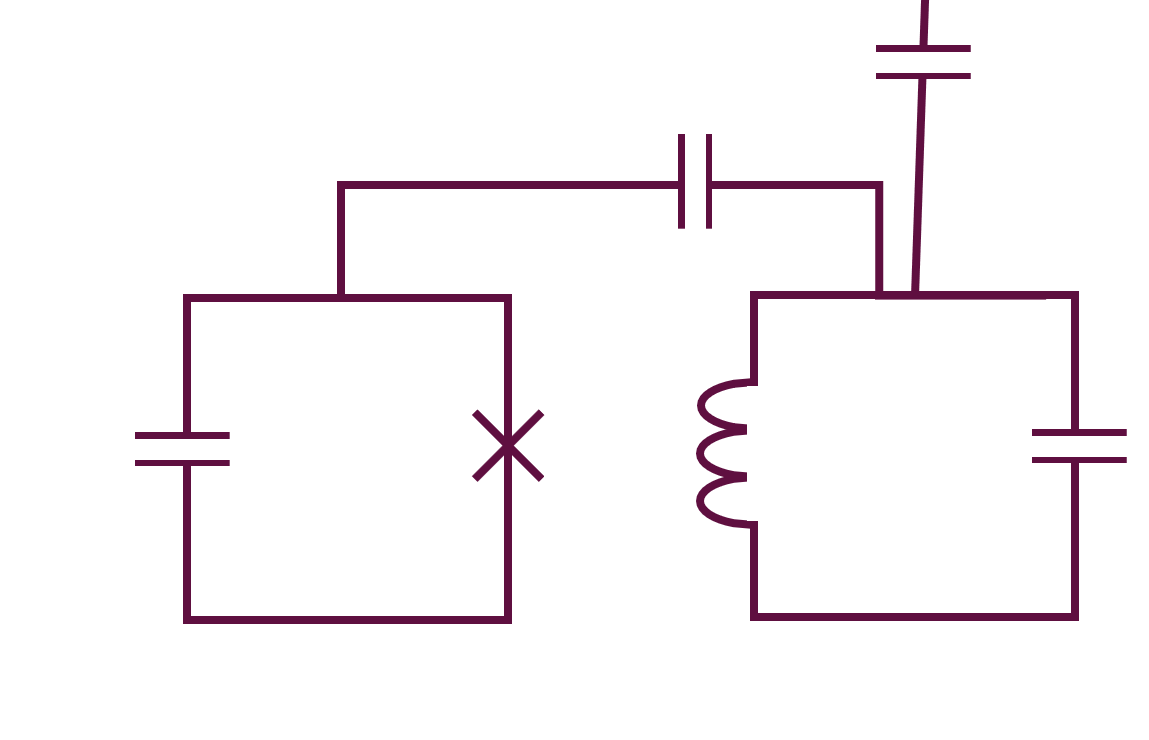
\includegraphics{Figs/Sections/computations_and_readout/qubit_resonator_feedline.png}
    \caption{A schematic of a Transmon coupled capacitatively to a resonator, which again is coupled to a feed line.}
    \label{fig:schematic_qubit_res}
\end{marginfigure}
\begin{equation}
    H_{int} = g n_c n_r 
\end{equation}
By using that $n_c \propto a + a^\dagger$ and $n_t \propto \sigma_+ + \sigma_-$ we obtain the Jaymes Cunning interaction:
\begin{equation}\label{eq:full_interaction_term}
    H_{int} = g (a + a^\dagger) (\sigma_- + \sigma_+)
\end{equation}
Where the factors of $n_c, n_t, C$ and the other constants are all absorbed into the coupling strength $g$ \cite{krantz_quantum_2019}. 


\subsection{Rotating Wave Approximation}
To optimize the computation time, it is beneficial to get rid of fast oscillating terms. First we choose to go into the interaction picture, where we try to cancel the time evolution of the non-interacting Hamiltonian.
\begin{equation}
    H_0 = \omega_r \; a^\dagger a + \omega_q\frac{\sigma_z}{2} 
\end{equation}
where the associated time evolution operator will be:
\begin{equation}
    \unitary(t) = e^{iH_0t}
\end{equation}
In the interaction picture, we will now have: $\ket{\psi} \rightarrow \unitary\ket{\psi}$ to counteract the fast oscillations from the $H_0$ term. The Hamiltonian will transform as: $H \rightarrow U(t) H \; U^\dagger(t)$. This yields the effective interaction Hamiltonian given by:
\begin{align*}
    H_{int}(t) = H_0 + g \left(e^{it(-\omega_r - \omega_q)} a \sigma_- + e^{it(\omega_r - \omega_q)} a^\dagger \sigma_-\right.  \\ 
    \left.e^{it(-\omega_r + \omega_q)} a \sigma_+ + e^{it(\omega_r + \omega_q)} a^\dagger \sigma_+\right)
\end{align*}
We now perform the rotating wave approximation, where we drop fast oscillating terms:
\begin{equation}
    H_{int}(t) \approx H_0 + g \left(e^{it\Delta}a^\dagger\sigma_- +  e^{-it\Delta}a\sigma_+\right)
\end{equation}
Here $\Delta = \omega_r - \omega_q$ is the detuning between the resonator and the transmon. Back in the Schrödinger picture, we get the interaction as \cite{blais_circuit_2021}:
\begin{equation}
    H_{S} = H_0 + g \left(a^\dagger\sigma_- +  a\sigma_+\right)
\end{equation}

\subsection{Dispersive Regime}\label{sec:dispersive_regime}
In most resonator-qubit systems, they are designed to have a dispersive interaction, that is:
\begin{equation}
    \lambda = \frac{g}{\Delta} \ll 1
\end{equation}
Here the system has nice properties for readout which we can analyze by doing some approximations. We can obtain a form of the Hamiltonian which is diagonal to first order in $\lambda$ by using the \textit{Schrieffer Wolff transformation}. For a Hamiltonian of type $H = H_0 + \lambda V$, the idea is to apply a transformation $\boldsymbol{D} = e^{\lambda S}$ to get: \footnote{Here we use, that the exponential of an operator is given by its power series: $e^{\lambda S} = \sum_n (\lambda S)^n / n!$ and $e^{-\lambda  S} = \sum_n (-1)^n (\lambda S)^n / n!$}
\begin{align*}
    H' = \boldsymbol{D}^\dagger H \boldsymbol{D} &= e^{-\lambda S} (H_0 + \lambda V) e^{\lambda  S} \\
    &= H_0 + \lambda V + \comm{\lambda S}{H_0 + \lambda V} + \frac{1}{2!} \comm{S}{\comm{S}{H}} + \dots
\end{align*}
Since $\lambda \ll 1$, we approximate the system by neglecting terms of second order or higher in $\lambda$. We can further diagonalize the Hamiltonian to first order if we choose $S$ such that $V + \comm{S}{H_0} = 0$. With a transmon dressed by a resonator, we choose the transformation given by:
\begin{equation}
    S = (a \sigma_+ - a^\dagger \sigma_-)
\end{equation}
Such that:\footnote{Where we can use the commutator relation $\comm{AB}{C} = A\comm{B}{C} + \comm{A}{B}C$ to find $\comm{a^\dagger a}{a^\dagger} = a^\dagger$ and $\comm{a^\dagger a}{a} = - a$. While $\comm{\sigma_z}{\sigma_+} = -2\sigma_+$ and $\comm{\sigma_z}{\sigma_-} = 2\sigma_-$.}
\begin{align*}
    \comm{H_0}{S} &= \comm{\omega_r a^\dagger a + \omega_q \sigma_z / 2}{a \sigma_+ - a^\dagger \sigma_-} \\
    &= - \omega_r \left(a^\dagger \sigma_- + a \sigma_+\right) - \frac12 \omega_q \left(2a^\dagger \sigma_- + 2 a \sigma_+ \right) \\
    &= -  (\omega_r + \omega_q)\left(a^\dagger \sigma_- + a \sigma_+\right) = - \Delta \left(a^\dagger \sigma_- + a \sigma_+\right) \\
    &= - \frac{g}{\lambda} \left(a^\dagger \sigma_- + a \sigma_+\right) = - V 
\end{align*}
This exactly leads to:
\begin{equation*}
    V + \comm{S}{H_0} = 0
\end{equation*}
While we get a new contribution to the Hamiltonian by:
\begin{align*}
    \comm{S}{V} &= \lambda g \comm{a^\dagger \sigma_- - a \sigma_+}{a^\dagger \sigma_- + a \sigma_+} \\
                &= \lambda g \left(a^\dagger a \sigma_- \sigma_+ - a a^\dagger \sigma_+ \sigma_-\right) \\
                &= 2 \lambda g \left(a^\dagger a \sigma_z + \frac12 \lambda g \sigma_+\sigma_-\right) \\
                &= \lambda^2 g^2 \ket{1}\bra{1} + 2 \chi a^\dagger a \sigma_z
\end{align*}
Here we have defined $\chi= g^2 / \Delta$ as the dispersive shift, which here is a measure of how much the resonator frequency moves depending on the state of the qubit. The $\lambda^2 g^2 \ket{1}\bra{1}$ is a contribution to the first excited state of the qubit and will normally just be absorbed into a new qubit frequency slightly shifted by resonator. The dispersive Hamiltonian now reads:
\begin{equation}\label{eq:dispersive_shift_tls}
    H = \left(\Tilde{\omega}_r a^\dagger a + \chi \sigma_z a^\dagger a \right)  + \frac12 \Tilde{\omega}_{01} \sigma_z
\end{equation}
Where the qubit and resonator frequency are altered to include the shift they impose on each other \cite{boissonneault_dispersive_2009}. To see the effect, one could drive the resonator at different frequencies and plot the expectation photon number $\expval{n}$ at the end for different qubit states. A result of such a simulation can be seen in \ref{fig:dispersive_two_level_qubit}. In this case, the width of the curves are dependent on the drive time, often one will however see them Lorentzian shaped, with a width determined by the lifetime of the photons in the resonator.
\begin{marginfigure}
    \centering
    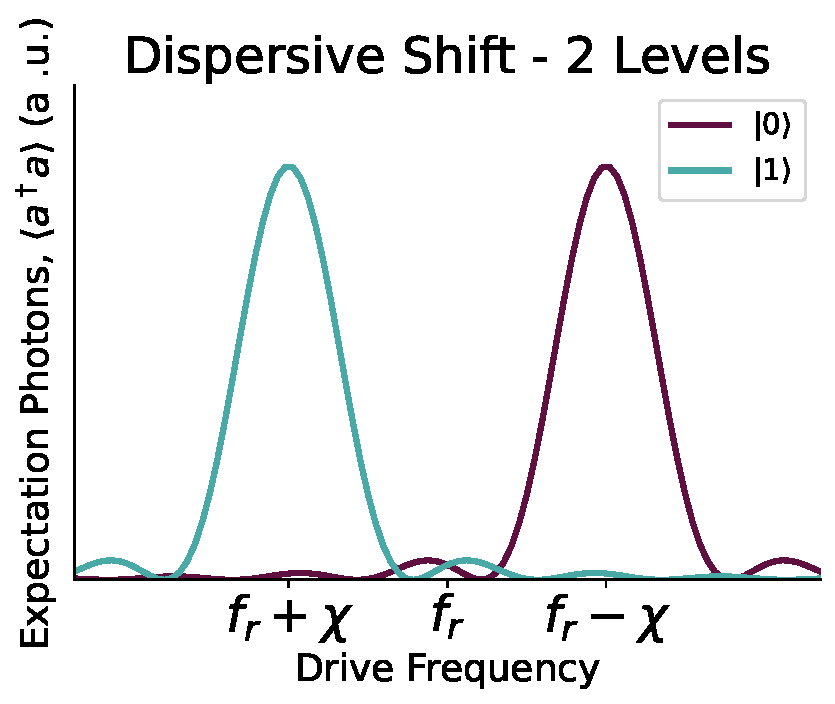
\includegraphics[]{Simulations/readout_simulations/dispersive_shift_2_level.pdf}
    \caption{Simulated driving of a qubit-resonator system using the dispersive approximation.}
    \label{fig:dispersive_two_level_qubit}
\end{marginfigure}

If we were to consider multiple levels of the qubit, the calculation require a  bit more work. This has been done in appendix \ref{appendix:} and leads to a general form of the Hamiltonian for a multi level qubit:
\begin{equation}\label{eq:multi_qubit_dispersive_hamiltonian}
    H' = \left(\omega_r + \sum_k \chi_k \ket{k}\bra{k} \right) a^\dagger a + \sum_k (\omega_k + \delta_k)\ket{k}\bra{k}
\end{equation}
Where the quantities are derived from a coupling matrix with elements $g_{ij} = g \mel{i}{n}{j}$ and the qubit energies as:
\begin{align}
    \chi_{ij} &= |g_{ij}|^2 \left(\frac{1}{\omega_{ij} - \omega_r} + \frac{1}{\omega_{ij} + \omega_r} \right) \\
    \delta_{ij} &= \frac{|g_{ij}|^2 }{\omega_{ij} - \omega_r} \\
    \chi_{i} &= \sum_j \chi_{ij} \\
    \delta_{i} &= \sum_j \delta_{ij} 
\end{align}
In this form, both the resonator frequency at the ground and first excited state of the qubit is shifted by an amount. This alters the effective dispersive shift between these two to\cite{krantz_quantum_2019}:
\begin{marginfigure}
    \centering
    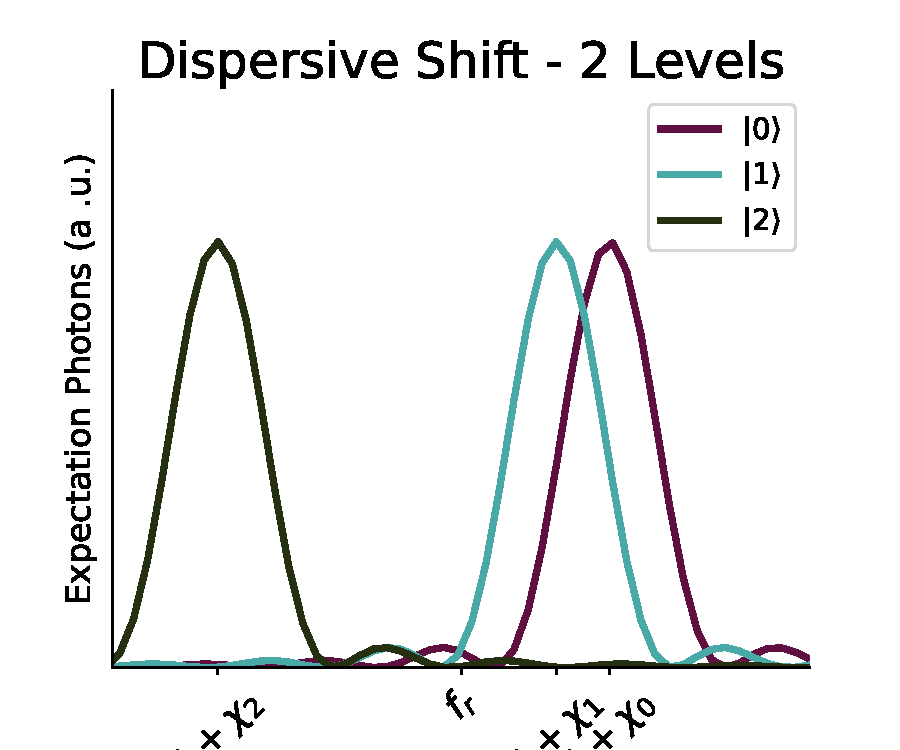
\includegraphics[]{Simulations/readout_simulations/dispersive_shift_3_level.pdf}
    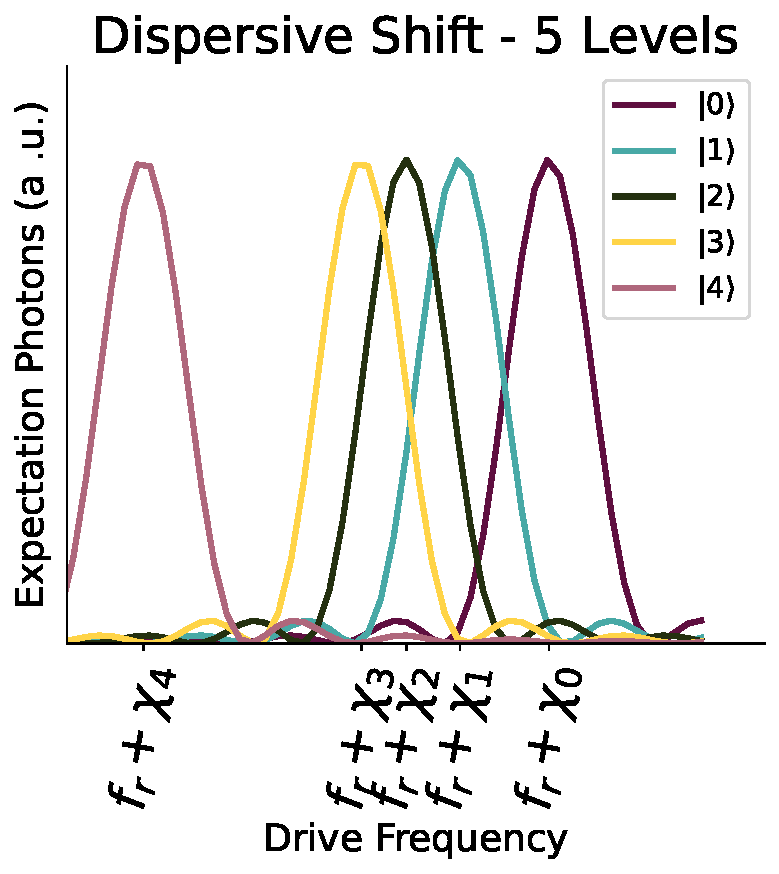
\includegraphics[]{Simulations/readout_simulations/dispersive_shift_5_level.pdf}
    \caption{Same simulating driving as figure \ref{fig:dispersive_two_level_qubit}, but with a 3 and 5 level qubit respectively.}
    \label{fig:dispersive_multi_level}
\end{marginfigure}
\begin{equation}\label{eq:chi}
    \chi \approx \chi_{01} + \chi_{12}/2 = - g_{01}^2/\Delta \left(\frac{1}{1 + \Delta / \alpha}\right)
\end{equation}
The effect can be seen in figure \ref{fig:dispersive_multi_level} where the second excited state moves the frequncy of the first much closer. This repeats when adding a third, fourth or higher excited state.
When deriving the equations the dispersive model, we neglect terms of order $\lambda^2$ or above. If we were to keep this term, it would have been multiplied with a $a^\dagger a$. If the mean photon number would have more than order $1 / \lambda^2$, it is no longer valid to throw the terms out. To be sure the dispersive model is a good approximation, one should therefore stay under a critical photon number, where $n_{\text{crit}} = \Delta^2 / 4 g^2$ \cite{krantz_quantum_2019}.
When calibrating our qubit in chapter \ref{chap:calibration}, we will find a critical photon number of $n_{\text{crit}} \approx 81$,and since we will be driving the resonator to around $\expval{n} \approx 21 \approx n_{\text{crit}} / 4$, this is well below the critical number. The dispersive approximation should therefore still provide a good model \cite{boissonneault_dispersive_2009}. 



\subsection{Readout Drive in the Dispersive Approximation}
When we perform a readout, we drive a capacitatively coupled line on the resonator like what we did with the qubit in section \ref{sec:qubit_control}. Choosing a driving pulse with a rectangular envelope and phase 0, we have a contribution to the Hamiltonian of the form:
\begin{equation}
    H_{drive} = \epsilon\cos(\omega_d t)(a + a^\dagger) = \frac{\epsilon}{2} \left(e^{i\omega_d t} + e^{-i\omega_d t}\right)(a + a^\dagger)    
\end{equation}
where $\epsilon$ is the amplitude of the drive and $\omega_d$ is the drive frequency. As with the last few times we encountered fast rotations, we now enter the rotating frame to cancel the rapidly oscillating terms. We choose the time dependent transformation:
\begin{equation}
    \unitary(t) = \exp\left(- i t \sum_k (\omega_k + \delta_k) \ket{k}\bra{k}\right) \otimes \exp \left(- i t \omega_d \;  a^\dagger a \right)
\end{equation}
To find effective Hamiltoninan:
\begin{equation}
    H_{eff} = \dot{i \mathcal{U}}{(t)}\unitary^\dagger(t)) + \unitary(t) H \unitary^\dagger(t)
\end{equation}
We find the contribution from the "centrifugal" term as:
\begin{equation}
    \dot{i \mathcal{U}}{(t)}\unitary^\dagger(t)) = - i t \sum_k (\omega_k + \delta_k) \ket{k}\bra{k} - it \omega_d \;  a^\dagger a
\end{equation}
The drive hamiltonian transforms as:
\begin{align*}
    H_{drive} &\to \unitary(t) H_{} \unitary^\dagger{t} \\
    &= \frac12 \epsilon (e^{i\omega_d t} + e^{-i\omega_d t}) \left[ \; \unitary(t)  (a + a^\dagger) \unitary^\dagger(t)\right] \\
    &= \frac12 \epsilon (e^{i\omega_d t} + e^{-i\omega_d t}) \left[ \;a e^{i \omega_d t} + a^\dagger e^{-i \omega_d t} \right]
\end{align*}
Neglecting the fast rotating terms ($\propto e^{\pm 2i\omega_dt}$), we get the effective drive Hamiltonian:
\begin{equation}
    H_{d, eff} = \epsilon(a + a^\dagger)
\end{equation}
Such that the total effictive Hamiltonian now becomes:
\begin{equation}
    H_{eff} =  \left(\omega_r - \omega_d + \sum_k \chi_k \ket{k}\bra{k}\right)a^\dagger a + \epsilon(a + a^\dagger)
\end{equation}
Which gives a nice time-independent Hamiltonian for m-level qubit which will prove ideal for simulation purposes. % Here we chose to have a $\cos$ pulse with no phase, but we could (like in section \ref{sec:qubit_control}) have chosen a phase $\phi$, to get the last term as $\cos(\phi)\epsilon(a + a^\dagger) + \sin(\phi)i\epsilon(a - a^\dagger)$. Since this is only a matter of a phase, the actual form used may vary throughout the thesis. \todo{Would be nice with some figures/physics here. Maybe comment on the approximations.}



\section{I-Q Phase Space}\label{sec:IQ_phase_space}
In the last section, we showed how the resonator experiences a state dependent shift of its frequency depending on the qubit. A valid way of doing readout is to drive the resonator at the frequency associated with $\ket{1}$. If the photon are now absorbed by the resonator, we can label the state "1". Often it is however beneficial to drive the resonators in between the two frequencies \cite{blais2004}. In this section, we will built up the tools for visualizing the two dimensional information in the IQ-plane which will allow us to understand why this is the case.

For a quantum harmonical oscillator, we represent the state by introducing the raising and lowering operator from the position and momentum: $a \propto x + ip$ and $a^\dagger \propto x - ip$. We can of course always measure $x$ or $p$ by representing them as $x \propto a + a^\dagger$ and $p\propto i (a - a^\dagger)$. Because of Heisenbergs uncertainty principle, we can however not know both of them at once. This is summed up in the between their uncertainties: $\sigma_x \sigma_p \geq 1/2$.  The same ideas can also be used to think about the state of the resonator. Here we define the \textit{quadrature operators} which also obey Heisenberg's uncertainty principle. They are defined  as\cite{knight}: 
\begin{equation}
    Q = a + a^\dagger \hspace{2 cm} I = i(a^\dagger - a)
\end{equation}

% In a quantum harmonic osci
% As a start, lets consider the quantum harmonic oscillator subject to $H = \omega^2  x^2 + p^2$ with proper definitions of $x$ and $p$ which properly satisfy $\comm{x}{p} = i$. To diagonalize the Harmonic Oscillator, one usually introduces the raising and lowering operator by:
% \begin{align}
%     &a \propto x + ip \hfill &a^\dagger \propto x - ip \\
%     &x \propto a + a^\dagger \hfill &p\propto i (a - a^\dagger)
% \end{align}
% Now, one can consider the harmonic oscillator either discretely in the $n = a^\dagger a$ eigenspace or in the continuous basis of $x$ and $p$. The same can be done with photons in a resonator. Where we consider the "quadratures" of the electric field, which we define as Q and I and are defined by the photon creation and annihilation operator in a way quite like the $x$ and $p$ operators of the harmonic oscillator \cite{knight}:


\subsection{Coherent States}
In a Harmonic Oscillator, the number states have expectation values $\expval{x} = \expval{p} = 0$. To get non-zero values of these expectation values, one is required to have superposition states with adjacent components. Example: $c_n\ket{n} + c_{n+1} \ket{n+1}$, which would satisfy $\expval{x} \propto \expval{a + a^\dagger} \neq 0$. The more natural states which would have position and momentum would be the eigenstates to the lowering operator:
\begin{equation}
    a \ket{\alpha} = \alpha \ket{\alpha}
\end{equation}
Where we can expand $\ket{\alpha}$ into the Fock basis. This gives us:
\begin{align}
    a \sum_n C_n \ket{n} =     \sum_{n = 1} C_n \sqrt{n} \ket{n - 1} = \alpha \sum_{n = 0} C_n \ket{n}
\end{align}
Here we can extract a relation between their coefficients:
\begin{equation}
    \sqrt{n} C_n = \alpha C_{n - 1}
\end{equation}
If we know $C_0$, we can now determine the rest of the series by:
\begin{equation}
    C_N = \frac{\alpha^n}{\sqrt{n!}} C_0 
\end{equation}
Ultimately, we can find an expression for the state $\ket{\alpha}$ in terms of the raising operator.
\begin{equation}
    \ket{\alpha} = C_0 \sum_n \frac{\alpha^n} {\sqrt{n!}} (a^\dagger)^n \ket{0}
\end{equation}
and $C_0$ is fonud from the normalization to be $C_0 = e^{- |\alpha|^2 / 2}$. Thus a coherent state is given as:
\begin{equation}
    \ket{\alpha} = e^{-|\alpha|^2 / 2} \sum_n \frac{\alpha^n}{\sqrt{n!}} \ket{n}
\end{equation}
Where each complex $\alpha$ corresponds to a coherent state. If $\alpha = 0$, we have the vacuum state which is the same as the vacuum Fock state $\ket{\alpha = 0} = \ket{n = 0}$. 



% \todo{Can we include the following}
% \begin{itemize}
%     \item The coherent states all have the lower limit on the Heisenbergs uncertainity principle.
%     \item When driving a coherent state with term like $a + a^\dagger$ it is a translation of the coherent state.
% \end{itemize}

% \begin{align}
%     1 &= |C_0|^2 \bra{0}\sum_{n, m}\frac{(\alpha^*)^m} {\sqrt{m!}} a^m \frac{\alpha^n} {\sqrt{n!}} (a^\dagger)^n \ket{0} \\
%     1 &= |C_0|^2 \sum_n \frac{|\alpha|^{2n} }{n!} = |C_0|^2 e^{|\alpha|^2} \\
%     |C_0|^2 &= e^{-|\alpha|^2}
% \end{align}
% \subsection{Overcompleteness / Properties of Coherent States}
% \textbf{This is probably relevant for the Q function} 

\subsection{Phase Space Representations}
With the coherent states we have a set of state that span a two-dimensional plane. We can use these to formulate a two dimensional pseudo-probability density function for values the values in $I$ and $Q$. This should take the Heisenberg uncertainity principle into account, such that the vacuum state for example should be a two dimensional Gaussian with standard deviation $\frac12$. Another desired property of this distribution should be the ability to express expectation values, $\expval{O} = \mel{\psi}{O}{\psi}$ in phase space. If we were to represent an operator in a coherent basis, it would take the form:
\begin{equation}
    O = \int d\alpha^2 O(\alpha, \alpha^*)\ket{\alpha}\bra{\alpha} 
\end{equation}
The expectation value $\expval{O}$ will now take the form: 
\begin{align*}
    \expval{O} &= \mel{\psi}{O}{\psi} \\
               &= \sum_n \bra{\psi} \int d\alpha^2 O(\alpha, \alpha^*)\ket{\alpha}\bra{\alpha} \ket{\psi}\\
               % &= \sum_n \bra{n} \int d\alpha^2 O(\alpha, \alpha^*)\ket{\alpha}\bra{\alpha} \ket{\psi}\bra{\psi} \ket{n} \\
               &= \int d\alpha^2 O(\alpha, \alpha^*) |\braket{\psi}{\alpha}|^2
\end{align*}
Here $|\braket{\psi}{\alpha}|$ takes the role of a probability distribution in the coherent phase space. To further ensure that the function is properly normalized, we must have the sum of all probabilities to equal 1. This is enforced by demanding that the expectation value of the identity is equal to 1. But since the set of coherent states are overcomplete (the fact that the integral is two dimensional, should be a hint), the identity has an extra factor of $1 / \pi$ \cite{knight}. 
\begin{align*}
    1 = \expval{\identity} &= \int d\alpha^2 \frac{1}{\pi} |\braket{\psi}{\alpha}|^2
\end{align*}
This gives us a pseudo-probability function given by: 
\begin{equation}
    Q(\alpha) = \frac{1}{\pi} |\braket{\psi}{\alpha}|^2
\end{equation}
This even works, when we have non-pure states represented by a density matrix (as we will soon introduce in sec \ref{sec:density_matrix_formalism}). Here it is called the Husimi $Q$-function and given by:
\begin{equation}
    Q(\alpha) =  \frac{1}{\pi} \mel{\alpha}{\rho}{\alpha}
\end{equation}
The $Q$-function is a powerful tool, which allows us to visualize some state in the phase space. Some common states like the vacuum state, a fock state or a coherent state can be seen in figure \ref{fig:Q_func_examples}.

\begin{marginfigure}[-12 cm]
    \centering
    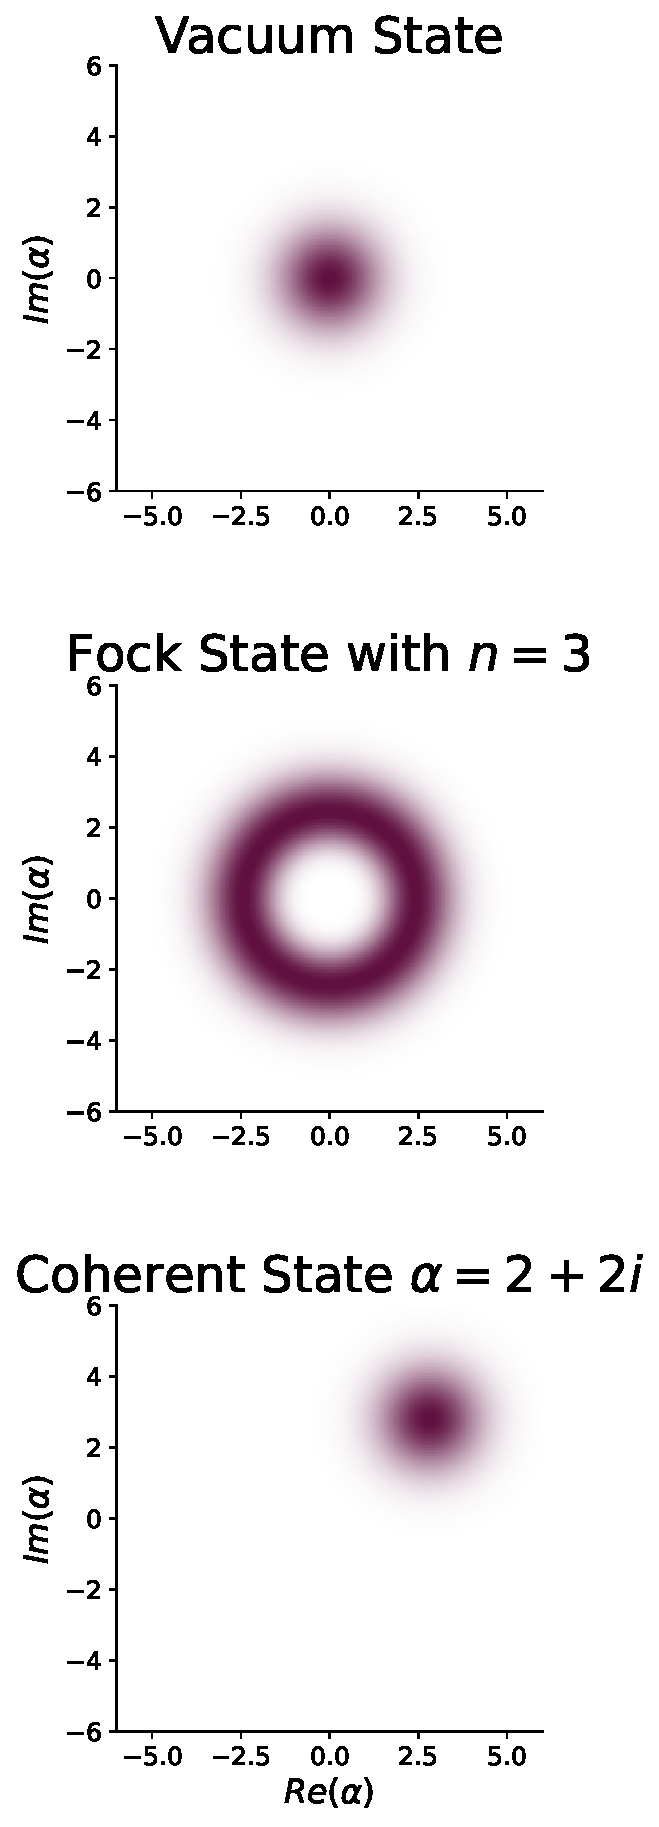
\includegraphics{Figs/Theory/Q_functions.pdf}
    \caption{Example of Different Q-functions for vacuum state, Fock state ($n = 3$) and a coherent state with $\alpha = 2 + 2i$.}
    \label{fig:Q_func_examples}
\end{marginfigure}

% \subsection{Common States *}
% Were we to solve the Hamiltonian in either the position or momentum basis, we would find that the ground state solution to be a Gaussian centered around the bottom of the square-potential and for higher states, we would have some multiplication with a Hermite Polynomial of corresponding order. This fact can be seen in figure \ref{fig:Q_func_examples} where the vacuum state is a 2D gaussian centered at the center (\textit{check validity of statement}). \\
% Now for the higher Fock states ($n = 3$ is shown), we see a ring, which is centered with an average radius of $n$. A good intuition for this is the energy conservation of the harmonic oscillator. If we were to measure the position $x=0$ of a harmonic oscillator with non-zero energy, it would certainly have a non-zero momentum. Of course in quantum mechanics this is smeared a bit by Heisenberg Uncertainty Principle.\\
% The coherent state described in the previous sections behaves like moving the vacuum around. The center of the distribution will be in $\alpha$.  

\subsection{The Driven Resonator in the IQ Plane}\label{sec:driving_resonator_iq_plane}
With the new formulation of Q-functions we can visualize the readout drive as a separation in the IQ plane. Let us explore what happens, when we drive the resonator while considering the qubit to be a two level system subject to the Hamiltonian:
\begin{equation}
    H_{eff} =  \left(\omega_r - \omega_d + \chi \sigma_z\right)a^\dagger a +\epsilon(a + a^\dagger)
\end{equation}
We can find the equation of motion of the operator $a$ in the Heisenberg picture \cite{sakurai_modern_2021}:
\begin{equation}
    \dot{a}(t) = i\comm{H_{eff}}{a} = -i\comm{\left(\omega_r - \omega_d + \chi \sigma_z\right)a^\dagger a + \epsilon(a + a^\dagger)}{a}
\end{equation}
And using the commutation relations, we find:
\begin{equation}
    \dot{a}(t) = -i \left(\left(\omega_r - \omega_d + \chi \sigma_z\right) a(t) - \epsilon\right)
\end{equation}
We now consider the resonator to be in a coherent state $\ket{\alpha}$ (initially we consider $\alpha(t=0) = 0$) and the qubit is in $\ket{k}$ with $k = 0,  1$. By looking at the expectation value of the operator, which will be the same in the Heisenberg and Schrödinger pictures, we get: % \cite{blais_circuit_2021}:
\begin{align}
    \dfrac{d}{dt} \bra{\alpha, k} a \ket{\alpha, k} &= \bra{\alpha, k}- i  \left(\omega_r - \omega_d \pm \chi \right) a(t) + i\epsilon\ket{\alpha, k} \nonumber \\
    \dfrac{d}{dt} \alpha(t) &= - i  \left(\omega_r - \omega_d \pm \chi \right) \alpha(t) + i\epsilon \label{eq:resonator_movement}
\end{align}
Which is a differential equation for the pointing vector $\alpha$. If we were to start in a coherent state, for example the vacuum state, the equation also tells us that we would stay in a coherent state. An example of driving the qubit-state-dependent resonator can be seen in figure \ref{fig:IQ_movement_without_kappa} where the drive is a both the frequency of $\ket{1}$ and in between the two. We should also notice that if we just use the absorption as a parameter (that is how far away the state is from origin), then we would in this case still get some signal if the qubit were in the $\ket{0}$ state. If we instead could readout the phase of $\alpha$ then we would have a much better way of separating the qubits in this case.

\begin{figure}
    \centering
    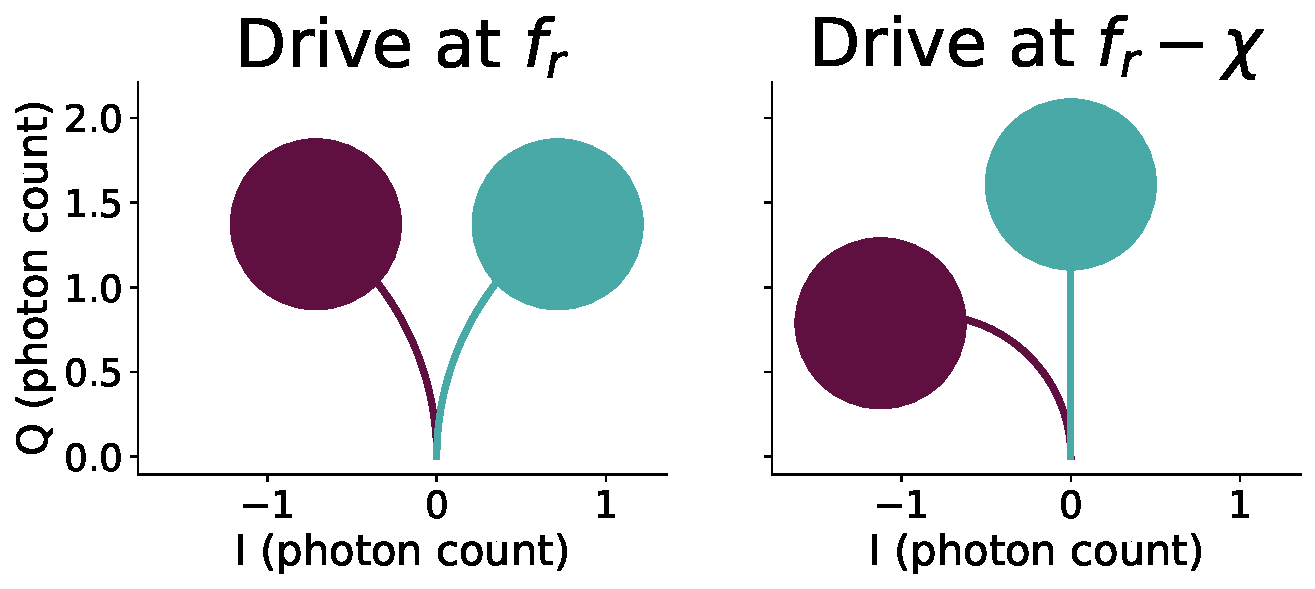
\includegraphics{Simulations/readout_simulations/IQ_movement_without_kappa.pdf}
    \caption{Driven resonator in the dispersive model where the qubit state is either $1$ or $0$ and we have used the realistic parameters for the constants in equation \ref{eq:resonator_movement} which we will calibrate in chapter \ref{chap:calibration}. The path of $I, Q$ coordinates are displayed along with the standard deviation of a half, which we have for coherent states in the IQ plane.}
    \label{fig:IQ_movement_without_kappa}
\end{figure}


% \begin{itemize}
%     \item When driving the resonator, we move it in the IQ-plane
%     \item What happens if we're slighly off resonant. We see a curve
%     \item Display the path of two qubit when we apply a drive inbetween the resonances. 
% \end{itemize}


% \vspace{1 cm}
% We now want to enter the rotating frame of the resonator. To make sure we also cancel the fast oscillating terms of the qubit, we choose to do the time-dependent transformation:
% \begin{equation}
%     \ket{\psi} \to \ket{\tilde{\psi}} = \mathcal{U}(t)\ket{\psi}
% \end{equation}
% In this basis, the Schrödinger equation becomes:
% \begin{align*}
%     i\partial_t \ket{\tilde{\psi}(t)} &= i \partial_t (\mathcal{U}(t) \ket{{\psi}(t)}) \\
%     &= i \dot{\mathcal{U}}(t)\ket{\psi(t)} + i \mathcal{U}(t) {\ket{\Dot{{\psi}}(t)}}
% \end{align*}
% And using $\ket{\dot{\psi}(t)} = i H \ket{\psi}$ and $\ket{\psi(t)} = \mathcal{U}^\dagger(t) \ket{\tilde{\psi}(t)}$:
% \begin{equation}
%     i \partial_t \ket{\Tilde{\psi}(t)}= \left[(\dot{i \mathcal{U}}{(t)}\unitary^\dagger(t) + \unitary(t) H \unitary^\dagger(t)\right]\ket{\tilde{\psi}(t)}
% \end{equation}
% Such that the effective Hamiltonian in the rotating frame is given as:
% It is now possible, to use this fact to simultaneously remove the time-dependence from the drive and remove the fast oscillating terms from the Qubit states. We now want to transform the resonator driving hamiltonian and the dispersive hamiltonian from Eq. \ref{eq:multi_qubit_dispersive_hamiltonian}. We choose: 
% Such that the effective Hamiltonian from the system gets the "centrifugal" contribution:
% While the Hamiltonian stays constant, since $\comm{H_{sys}}{\unitary(t)} = 0$:
% \begin{equation}
%     \unitary(t) \; H_{sys} \; \unitary^\dagger(t) = H_{sys}
% \end{equation}